\section{Experiments}
\label{sec:experiments}

% ===== Figure & table includes for the TCI paper (generated 2026-09-30) =====
% Requires: \usepackage{graphicx}, \usepackage{booktabs}

% === Fig 1: hero triptych (double column) ===
\begin{figure*}[t]
    \centering
    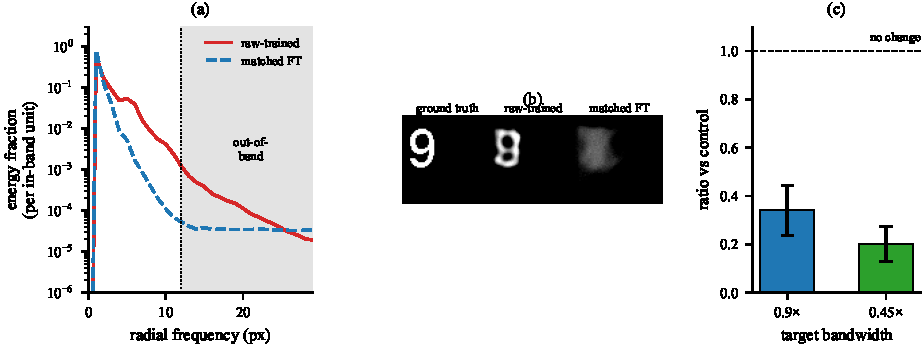
\includegraphics[width=0.95\textwidth]{figures/fig1_hero.pdf}
    \caption{Training-target bandwidth controls spectral fabrication. (a) Out-of-band energy is the reconstruction spectral energy outside the measured MTF support (shaded, vertical dotted line at the support radius); from an identical initialization, the raw-trained model keeps substantially more energy in this region (3$\times$ at the band edge) than the model fine-tuned against bandwidth-matched targets. (b) Reconstructions: the bandwidth-matched model suppresses out-of-band fabrication at the cost of visibly smoother (band-limited) output, which is the correct behavior under the measured information support; the raw-trained model restores sharper structure partly by inventing out-of-band content. (c) Suppression ratio of fine-tuned to compute-matched control out-of-band energy across both architectures and all seeds. Out-of-band energy is a fabrication proxy, not a perceptual metric.}
    \label{fig:hero}
\end{figure*}

% === Fig 2: paired control (single column) ===
\begin{figure}[t]
    \centering
    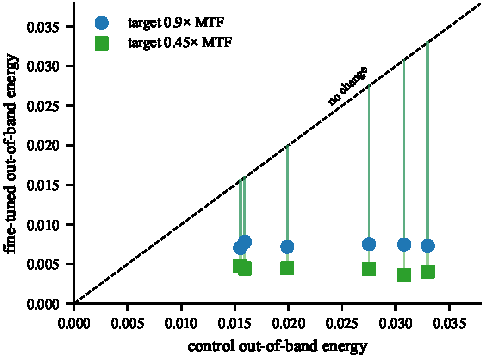
\includegraphics[width=0.48\textwidth]{figures/fig2_paired_control.pdf}
    \caption{Paired fine-tune versus compute-matched control (identical initialization; equal extra optimization). Each segment connects a unit's control value (on the no-change line) to its fine-tuned value. Matched-target ratio $0.34\pm0.11$ and half-target $0.20\pm0.08$; all 6/6 units reduce (one-sided sign test $p\approx0.016$).}
    \label{fig:paired}
\end{figure}

% === Fig 3: capacity (single column) ===
\begin{figure}[t]
    \centering
    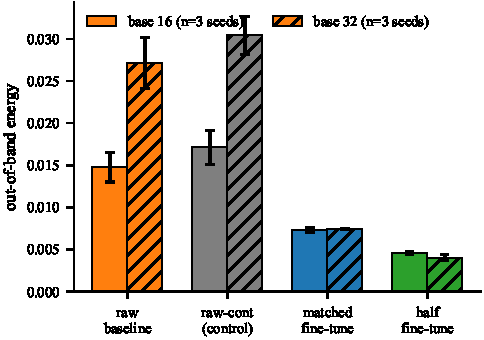
\includegraphics[width=0.48\textwidth]{figures/fig3_capacity.pdf}
    \caption{Out-of-band energy by arm for the two tested capacities. In the two tested capacities, the larger network fabricates more in the raw-baseline and control arms and admits stronger suppression under bandwidth-matched fine-tuning; described as an observed trend, not a scaling law. Error bars: std over 3 seeds.}
    \label{fig:capacity}
\end{figure}

% === Fig 4: trade-off (single column) ===
\begin{figure}[t]
    \centering
    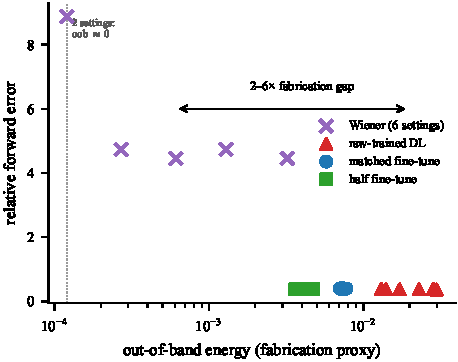
\includegraphics[width=0.48\textwidth]{figures/fig4_tradeoff.pdf}
    \caption{Fabrication versus forward fidelity. Wiener reconstructions (6 regularization/support settings) constrain out-of-band energy below the raw-target and matched arms in every cell (the half-bandwidth arm approaches the Wiener range) but operate at a roughly $1.4\times$ (${\sim}40\%$) worse relative forward error --- the learned arms therefore occupy a distinct operating point rather than dominating. Two Wiener settings with negligible out-of-band energy are drawn at the axis floor.}
    \label{fig:tradeoff}
\end{figure}

% === Fig 5: robustness (double column) ===
\begin{figure*}[t]
    \centering
    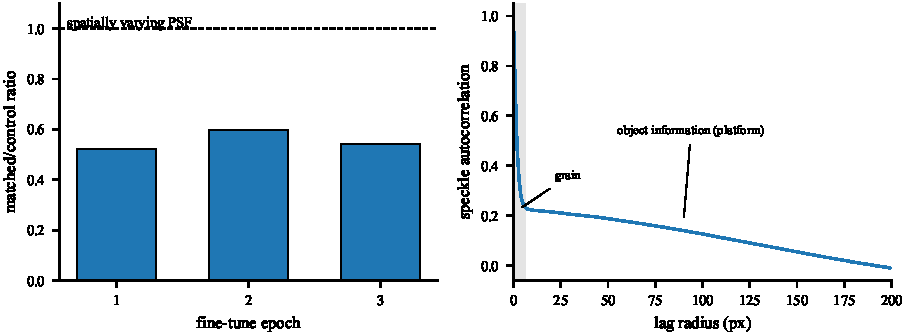
\includegraphics[width=0.92\textwidth]{figures/fig5_robustness.pdf}
    \caption{Left: the matched/control out-of-band ratio under a position-dependent (spatially varying PSF) forward operator remains stable across fine-tune epochs --- the suppression effect does not rely on shift-invariance. Right: measured speckle autocorrelation from the public experimental dataset (DSC): a sub-pixel grain peak superposed on a wide platform that carries object information out to $\sim$190\,px lag --- the real-data structure our protocol targets; quantitative real-data reconstruction is left to future work (see text).}
    \label{fig:robustness}
\end{figure*}

% === Table 1 ===
\begin{table}[t]
\centering
\small
\caption{Out-of-band energy (fabrication proxy) and band-limited PSNR across arms; mean$\pm$std over 6 units (2 architectures $\times$ 3 seeds). The paired block reports fine-tune-to-control ratios within units.}
\label{tab:main}
\begin{tabular}{lcc}
\toprule
Arm & Out-of-band energy & PSNR (dB) \\
\midrule
Raw baseline (20 ep) & $0.0210 \pm 0.0073$ & $16.5 \pm 0.4$ \\
Bandwidth-matched baseline (20 ep) & $0.0066 \pm 0.0006$ & $31.7 \pm 1.3$ \\
Half-bandwidth baseline (20 ep) & $0.0036 \pm 0.0004$ & $22.1 \pm 1.2$ \\
Raw-continued control (+4 ep) & $0.0238 \pm 0.0077$ & $16.4 \pm 0.5$ \\
Matched fine-tune (4 ep) & $0.0074 \pm 0.0003$ & $29.8 \pm 0.9$ \\
Half fine-tune (4 ep) & $0.0043 \pm 0.0004$ & $21.8 \pm 0.2$ \\
\midrule
\multicolumn{3}{l}{Paired (fine-tune vs.\ control, within unit)} \\
Matched fine-tune ratio & $0.34 \pm 0.11$ & reduced 6/6 \\
Half fine-tune ratio & $0.20 \pm 0.08$ & reduced 6/6 \\
\bottomrule
\end{tabular}
\end{table}



\subsection{Baselines and the reference-dependence of fidelity}
\label{sec:baselines}

Table~\ref{tab:main} summarizes all arms. The three from-scratch baselines (20 epochs each) show the expected monotone ordering in fabrication: the raw-target model reaches $\oob = 0.0210 \pm 0.0073$, the bandwidth-matched model $0.0066 \pm 0.0006$ ($3.2\times$ lower), and the half-bandwidth model $0.0036 \pm 0.0004$ ($5.9\times$ lower). The band-limited PSNR ordering, however, inverts: the matched model scores $31.7$~dB, well above the raw model's $16.5$~dB and the half model's $22.1$~dB. The inversion is not paradoxical: PSNR is computed against a reference low-pass filtered at the matched bandwidth, and the raw model's out-of-band energy is penalized twice under that reference---once as fabrication, and once because the reference contains no such energy to match. This is why the protocol reports band-limited PSNR as a secondary, reference-dependent quantity and uses the no-reference forward-consistency endpoint for the causal comparison: the ranking of models under a reference-based fidelity metric depends on the bandwidth of the reference, and a benchmark result quoted without its reference bandwidth is under-specified.

\subsection{The causal intervention: fine-tuning versus compute-matched control}
\label{sec:main-control}

Fig.~\ref{fig:paired} shows the central result. Each segment connects one unit's control value (the continuation arm, on the no-change line) to the same unit's fine-tuned value, so every segment is a paired within-unit comparison under identical initialization and identical additional optimization. The matched-target fine-tune reduces out-of-band energy to a ratio of $0.34 \pm 0.11$ of its control, and the half-target fine-tune to $0.20 \pm 0.08$; all six units reduce in both settings (one-sided sign test $p \approx 0.016$), and the pre-registered criterion (ratio $< 0.8$) is met with margin. The model trained from scratch on matched targets reaches the same low fabrication level, while the compute-matched control moves in the \emph{opposite} direction: four additional epochs on the raw target increase fabrication from $0.0210$ to $0.0238$ on average across units (about $13\%$); the continuation is not a passive arm that merely freezes.

The no-reference endpoint rules out the trivial explanation that suppression is achieved by degrading the reconstruction into smoothness. The relative forward consistency of the matched fine-tune changes by a mean paired difference of $+0.026$ on a $0.36$--$0.40$ baseline---a small relative increase that bounds the fidelity cost of the suppression at roughly 7\% of the baseline forward error (the half-bandwidth \emph{baseline} sits at a distinct operating point, up to $0.47$, and is excluded from this comparison range). Fabrication suppression and measurement agreement are therefore close to unchanged rather than traded against each other, and the half-target arm moves by only $+0.006$. Fig.~\ref{fig:hero}(b) shows the qualitative behavior behind these numbers: at the matched bandwidth, the fine-tuned reconstruction is visibly smoother than the raw model's, and that smoothness is the correct band-limited behavior---the raw model's extra apparent structure is largely content the measurement cannot certify.

\subsection{Fabrication grows with capacity}
\label{sec:capacity}

Fig.~\ref{fig:capacity} splits the arms by network width. In the two tested capacities, the larger network (base 32) exhibits higher raw fabrication: $0.027$ versus $0.015$ in the raw baseline, and $0.030$ versus $0.017$ in the control. Suppression is correspondingly stronger for the larger network: the matched fine-tune ratio is $0.25$ for base 32 versus $0.44$ for base 16. These contrasts are point estimates over three seeds per width (per-arm variability in Table~\ref{tab:main}). Read together with Sec.~\ref{sec:wiener}, the pattern is consistent with the informal hypothesis that extra capacity is spent, in part, on fabricating content beyond the measurement---and that bandwidth-matched targets reclaim that capacity for in-support reconstruction. We state this as an observed trend across the two tested widths, not as a scaling law; three or more capacity points would be required to establish the functional form.

\subsection{The Wiener anchor: a trade-off, not a defeat}
\label{sec:wiener}

How much fabrication is avoidable in principle? A Wiener filter with the known PSF is the optimal linear reconstruction under the protocol's noise model, and it cannot fabricate out-of-band content: its output energy outside the measured support is bounded by its regularization. Across a grid of six regularization/support settings, the Wiener reconstruction's out-of-band energy stays in $0.0003$--$0.0032$---$2$--$6\times$ below the raw-target and matched arms in every cell, while the half-bandwidth arm approaches the Wiener range (the worst Wiener cell is within ${\sim}1.1\times$ of the half arm's mean); two settings drive it to numerical zero (Fig.~\ref{fig:tradeoff}). The same grid, however, shows the price: evaluated under the same relative-forward-error definition with an optimal scalar rescaling of its output (a fair comparison, since a raw Wiener estimate is not amplitude-calibrated), Wiener's relative forward error is $0.52$--$0.55$, versus $0.36$--$0.40$ for the learned arms---roughly $40\%$ higher. The linear baseline is spectrally conservative because it remains under-fitted: it fails to re-explain its own measurement by about $1.4\times$ more than the learned arms. The learned arms therefore occupy a distinct operating point in the (fabrication, forward-fidelity) plane rather than dominating or being dominated. The bandwidth-matched fine-tune moves a learned model toward, but not to, the linear regime---the honest summary of the trade-off is that fabrication can be controlled by at least $3\times$ at a fidelity cost bounded at about $7\%$ of the baseline forward error, not that it can be eliminated for free.

\subsection{Robustness to a position-dependent forward operator}
\label{sec:svpsf}

The protocol above assumes a shift-invariant PSF. Real scattering systems violate this: the PSF varies across the field, and the memory-effect range is finite. To test whether the suppression effect rides on the shift-invariance idealization, we replace the single PSF with a position-dependent operator: four independently seeded PSFs blended by feathered quadrant masks, so the forward operator changes with position while its local statistics stay matched. Under this operator, retraining the same arms reproduces the effect: the matched-to-control out-of-band ratio is $0.52$, $0.60$, $0.54$ at one, two, and four fine-tune epochs---stable across optimization length and clearly separated from the no-change line (Fig.~\ref{fig:robustness}, left). These levels come from a single-seed robustness configuration with a different forward operator and are therefore not directly comparable to the multi-seed main result of Sec.~\ref{sec:main-control}; the quantity this experiment establishes is the \emph{stability and sign} of the suppression under a broken shift-invariance assumption. A companion fine-tune-length sweep under the shift-invariant protocol shows the same stability ($0.52$, $0.49$, $0.50$), which rules out a transient-optimization explanation for the suppression. The mechanism therefore does not require exact shift invariance.

\subsection{Negative control: no class boundary in transfer loss}
\label{sec:negative}

The field's standard training protocol is defined over ``same-class'' diffusers \cite{li2018deep}. If cross-diffuser transfer loss were governed by a genuine class boundary, protocol design could target class membership; if not, the label is a convenience and quantitative statistics---reported distance, measured bandwidth---should replace it. We trained twelve decoders on twelve synthetic diffusers arranged as an orthogonal grid over three factors (pupil radius, phase-height distribution, phase-spectrum smoothness), evaluated the full $12\times12$ transfer matrix on identical test objects, and fitted each of three statistical distances (height-map Wasserstein, speckle power-spectrum Jensen--Shannon, patch-level MMD) against the paired transfer losses. Under all three metrics, a segmented (changepoint) fit fails to beat a smooth monotone fit by the model-selection criterion ($\Delta\text{BIC} = \text{BIC}_{\text{segmented}} - \text{BIC}_{\text{smooth}} = -1.4, +5.6, +3.3$ respectively; positive values favor the smooth fit, and none clears the $-10$ threshold that would favor a changepoint), and permutation tests put the changepoint's apparent gains inside the null distribution ($p = 0.08, 0.91, 0.41$). Two of the twelve decoders (strong-scattering binary-phase diffusers) converge to partially object-independent solutions for out-of-family inputs; we disclose this and verify that the conclusion is insensitive to it---excluding both affected decoders leaves every metric inside the null distribution ($\Delta$BIC ranges from $-1.1$ to $+0.6$, permutation $p = 0.11$--$0.18$). Transfer loss varies smoothly with distance; there is no boundary to find. One further caution: the largest observed losses (up to $15.0$~dB) occur where a single distance is smallest but another factor differs---each distance is blind to the factors it does not measure---so a scalar law would need the joint distance, and we report the negative control as evidence for protocol-level reporting rather than as a claimed law. The full matrix and fit details are deferred to the supplementary material.
